%% Thresholds That Travel -- anonymous submission, ACM ASIA CCS 2027 (sigconf).
%% Converted from manuscript/thresholds_that_travel_draft_v0_1.md (draft v0.1, revised
%% after review/review_report.md). Every number is reproduced exactly as written in that
%% draft; nothing was re-rounded or recomputed.
%% Anonymization: author block, ORCID, repository links and the authors' own artifact DOIs
%% are removed; the artifact is cited by its anonymous.4open.science copy (contribution 5 and the
%% Open science appendix).
%% Third-party dataset DOIs (HyGrid-ICS, BATADAL, voraus-AD) are retained deliberately.
\documentclass[sigconf,review,anonymous]{acmart}

\settopmatter{printacmref=false}
\setcopyright{none}
\renewcommand\footnotetextcopyrightpermission[1]{}
\pagestyle{plain}

\usepackage{booktabs}
\usepackage{array}
\usepackage{tabularx}
\newcolumntype{L}{>{\raggedright\arraybackslash}X}
\newcolumntype{C}{>{\centering\arraybackslash}X}
\setlength{\emergencystretch}{2em}  % lets lines with unbreakable names (tracker\_slow) stretch
\usepackage{graphicx}
\usepackage{url}
\usepackage{placeins}  % \FloatBarrier before the conclusion keeps every float ahead of the references

% Ten full-width floats in roughly eight pages: with the class defaults the float queue jams and
% the last figures land after the references. Same settings as the USENIX copy.
\renewcommand{\topfraction}{0.9}
\renewcommand{\dbltopfraction}{0.9}
\renewcommand{\textfraction}{0.07}
\renewcommand{\floatpagefraction}{0.75}
\renewcommand{\dblfloatpagefraction}{0.75}
\setcounter{topnumber}{3}
\setcounter{dbltopnumber}{3}
\setcounter{totalnumber}{5}

\acmConference[ASIA CCS '27]{ACM ASIA Conference on Computer and
  Communications Security}{July 12--16, 2027}{Macau, China}
\acmISBN{}
\acmDOI{}

\begin{document}

\title{Thresholds That Travel: Adaptive Alarm Thresholds Let Attacks Through in
  ICS Anomaly Detection}

%% Author block removed for double-blind review.
\author{Anonymous Author(s)}

\begin{abstract}
Anomaly detectors for industrial control systems (ICS) raise an alarm when a score crosses a
threshold. The threshold is calibrated on clean data and must then hold a false-alarm budget
for months, so deployments often let it adapt: they recalibrate it daily, track a running
quantile, or refit an extreme-value tail as data arrive. Each rule learns from part of its input,
and we ask what happens when attacks land there.

In three pre-registered studies on data that no earlier analysis of ours had opened, a symmetric
quantile tracker lost attacks that a frozen threshold caught: 20 of HAI 20.07's 38 against 36
(difference $-0.42$, 95\% interval $[-0.58, -0.26]$), 6 of BATADAL's 14 against 14
($[-0.79, -0.29]$) and, on the Tennessee Eastman process, 66 of the 104 attacks that follow another
attack in their run against 104 ($[-0.47, -0.27]$). On the first attack of a run the two were equal
(116 of 141 each). A tracker calibrated to HAI 20.07's false-alarm rate needs 23 exceedance-free hours
to undo one minute above its threshold, whatever its step size. Under a stricter count, in which an
alarm must begin inside the attack (registered on Tennessee Eastman, post-hoc on the other two), the
loss holds on BATADAL but not on HAI 20.07 or Tennessee Eastman, where later attacks arrive inside
alarms already running; that failed the third study's primary rule. On a fourth dataset, ProvICS,
whose monitor was in alarm for 44\% of the unlabelled time, the tracker lost nothing.

Deliberate poisoning is cheaper. On 56 sealed attack-free Tennessee Eastman runs (registered), a day of
two-minute nuisance alarms left the tracker catching none of 56 later, just-detectable attacks; pulses
shorter than what a rule counts as an event did the same to a recalibration that leaves alarm episodes
out; and an attacker who held the score just under the current threshold left a standard SPOT threshold
catching 16 of 56 attacks a quarter above the calibrated threshold. The frozen threshold caught all 56 each time and ran at 0.98 times its false-alarm
budget over 280 attack-free days. A threshold that only tightens itself cannot miss an event the frozen
threshold catches, and a ceiling at $\kappa$ times the calibrated threshold confines every one of these
attacks to events at or below the ceiling. We argue that an alarm threshold may tighten itself but should
loosen only inside a fixed band or with operator approval, and we release the registrations, ledger and
code.
\end{abstract}

\keywords{industrial control systems, anomaly detection, adaptive thresholds, poisoning,
  extreme value theory, pre-registration}

\maketitle

\section{Introduction}

A process-monitoring anomaly detector has two parts: a score that grows when the plant behaves
unlike its normal operation, and a threshold that turns the score into alarms. Most of the
research effort goes into the score. The threshold is usually set once, on held-out normal data,
to meet a false-alarm budget, and then expected to hold that budget on a plant that drifts:
sensors age, seasons change load, and operators retune loops. When it does not hold, the standard
remedies adapt the threshold online. Daily recalibration re-estimates a quantile on the last day
of data. Online quantile tracking, the mechanism behind adaptive conformal
inference~\cite{gibbs2021aci}, nudges the threshold up after every exceedance and down otherwise.
Streaming peaks-over-threshold methods (SPOT and DSPOT~\cite{siffer2017spot}) refit a generalised
Pareto tail as new values arrive, and the nonparametric dynamic threshold of
Telemanom~\cite{hundman2018telemanom} recomputes its level on a trailing window.

Each of these rules learns from part of its input. Trackers and recalibration learn from the
values that exceed the threshold. SPOT and DSPOT discard values above their alarm level but learn
from values between a base level and the alarm level. A frozen threshold learns from nothing after
calibration. We call the part of the score range a rule learns from its \emph{learning region},
and the question of this paper is what happens when an attack, or an attacker, lands in it.

The answer depends on the region, and none of the rules we tested that can raise their own
threshold is safe:

\begin{itemize}
\item \textbf{Rules that learn from exceedances are poisoned by real attacks.} An attack is a long
  exceedance, so a tracker raises its threshold during the attack and stays high afterwards. The
  next attack then arrives under an inflated threshold. On fresh HAI 20.07 data the tracker missed
  18 of 38 attacks, 16 of them attacks the frozen threshold caught; on BATADAL it missed 8 of 14, all
  caught by the frozen threshold; on Tennessee Eastman it missed 38 of the 104 attacks that follow
  another attack and no more than the frozen threshold among first attacks. No adversarial planning is
  needed; the attacks in the recording did it.
\item \textbf{The same rules can be poisoned on purpose and loudly.} Twelve two-minute pulses a
  day, the kind of nuisance alarm operators learn to acknowledge, raised these thresholds enough to
  hide a later attack that a frozen threshold caught every time (registered on sealed attack-free
  Tennessee Eastman runs; exploratory on HAI).
\item \textbf{Rules that refuse to learn from alarms can be poisoned silently.} An attacker who
  reads the current SPOT or DSPOT threshold and holds the score just under it feeds every sample
  into the fitted tail. The tail extends, the threshold rises, and the attacker follows it up. At the
  score level the campaign usually raises no alarm (none in 51 of the 56 registered placements). A
  standard SPOT then caught 16 of 56 later attacks a quarter above the calibrated threshold on the
  sealed Tennessee Eastman runs, against 56 without the campaign (registered).
\item \textbf{Rules that leave alarms out of their update can be poisoned below their notice.} A
  recalibration that excludes alarm episodes must decide what an episode is. Pulses shorter than its
  event length do not count, so it learns from them (registered).
\end{itemize}

A threshold that only tightens itself cannot be pushed above the frozen threshold by any of these,
so it keeps the frozen threshold's recall by construction (Section~\ref{sec:memory}). Its cost is extra
false alarms. A ceiling at $\kappa\tau_0$ extends the guarantee to rules
that loosen: no poisoning can hide an event above the ceiling. Loosening beyond it is left to an
operator, and that step carries no such guarantee.

\paragraph{Method}
Three studies were registered, each before any test row or label of its datasets was read: tt1 (HAI
20.07, HyGrid-ICS, voraus-AD), tt1b (BATADAL) and tt1d (Tennessee Eastman, ProvICS; for these the
dataset documentation, the file names and the header lines of the label files were read first). A ledger records every access to recorded attack data, the analysis harness refuses to
run if any frozen source file changed after registration, and it computes the registered gates
itself. The rules and the attack designs came from development on three earlier HAI releases whose
attacks had already been used; we report how the claim changed during development, including two
hypotheses we dropped. Extensions run after the registered finals are labelled exploratory.

\paragraph{Contributions}
\begin{enumerate}
\item Three registered studies of threshold rules on six never-opened datasets (hardware-in-the-loop
  and simulated plants, an industrial robot), reporting every registered outcome, including three
  failed primary rules and one dated amendment
  (Sections~\ref{sec:registered} and~\ref{sec:replications}).
\item Evidence that exceedance-learning thresholds lose recall on real attacks because earlier
  attacks inflate them: registered on HAI 20.07, BATADAL and Tennessee Eastman, where the tracker's
  loss falls on attacks that follow attacks and not on the first attack of a run. Under a stricter
  onset count (registered on Tennessee Eastman, post-hoc elsewhere) the loss survives on BATADAL only,
  and ProvICS shows none.
\item A learning-region analysis of adaptive thresholds: how long the tracker and daily
  recalibration remember an exceedance (Section~\ref{sec:memory}), and a matching attack for each
  class, registered on sealed attack-free runs: loud pulses for exceedance learners, a closed-loop
  frog-boiling attack for extreme-value learners, and sub-event pulses for rules that leave alarms
  out (Section~\ref{sec:replications}).
\item A design rule, supported by these results: thresholds may tighten themselves; loosening needs
  a ceiling or a human (Section~\ref{sec:design}).
\item The registration, access ledger, harness and verifier, in the anonymized artifact at
  \url{https://anonymous.4open.science/r/thresholds-that-travel-artifact-579B/}.
\end{enumerate}

\section{Background and related work}

\paragraph{ICS anomaly detection}
Process-level detectors learn normal behaviour from sensor and actuator traces and flag deviations:
model residuals, autoencoder reconstruction errors, or statistical bounds. Public testbed recordings
with labelled attacks (SWaT~\cite{goh2016swat}, WADI~\cite{ahmed2017wadi},
BATADAL~\cite{taormina2018batadal}, and the HAI releases: HAI 1.0 (20.07)~\cite{shin2020hai}, 21.03
\cite{shin2021hai}, later releases in the dataset repository) are the usual benchmarks. Evaluations
usually fix one threshold per detector, chosen on clean data, by an offline peaks-over-threshold
fit~\cite{su2019omni}, or, less defensibly, on the test labels. Wu and Keogh~\cite{wu2023benchmarks}
list further benchmark pitfalls.

\paragraph{Threshold rules}
Static thresholds meet a quantile or false-alarm budget on clean data. Adaptive variants recalibrate on
a trailing window, track a target exceedance rate online~\cite{gibbs2021aci}, fit an extreme-value tail
and update it per observation (SPOT, and DSPOT for drifting streams~\cite{siffer2017spot}), or
recompute a level on a trailing window of smoothed errors~\cite{hundman2018telemanom}. Game-theoretic
time-varying thresholds~\cite{ghafouri2016thresholds} are precomputed, not learned from the stream.
Alarm-management practice treats nuisance and chattering alarms as a condition to eliminate, with
explicit alarm-rate targets, and routes changes to an alarm through authorised management of
change~\cite{isa182, eemua191}; operators who acknowledge nuisance alarms without investigating them are
the failure mode our pulse campaigns exploit.

\paragraph{Poisoning and stealthy attacks}
Rubinstein et al.~\cite{rubinstein2009antidote} showed that slowly growing (``boiling frog'') poisoning
of a weekly retrained PCA detector, whose threshold is re-estimated with it, can stop it flagging a
later attack. Kloft and Laskov~\cite{kloft2010online, kloft2012security} showed that bounding the
false-positive rate limits poisoning of online centroid detectors. Chan-Tin et
al.~\cite{chantin2009frog, chantin2011frog} described frog-boiling against outlier rejection in network
coordinate systems: every update stays within the rejection threshold while the system drifts. In ICS,
Kravchik and Shabtai~\cite{kravchik2020frog} found an autoencoder on SWaT physical-state data resistant
to poisoning, but later work poisoned online-retrained ICS detectors with sub-threshold samples and
proposed lowering the threshold as mitigation~\cite{kravchik2021poisoning}, and Seo
et al.~\cite{seo2026retraining} poisoned a drift-adaptive SWaT detector through its retraining step,
evading its drift detector until the retrained threshold cut precision from 0.91 to 0.24. Erba
et al.~\cite{erba2020concealment} concealed attacks from reconstruction-based detectors by manipulating
sensor readings. Attackers who hold a detection statistic just under a fixed threshold are standard in
control security~\cite{cardenas2011process, urbina2016stealthy}. Hong~\cite{hong2026boiling} studied
gradual drift against world-model monitors in simulation, without attacks or adaptive thresholds. These
works target the model or the score, or assume a fixed threshold. We target the adaptive threshold rule
and show that it can fail even when the model is not poisoned.

\paragraph{Distribution shift and calibration}
Adaptive conformal inference and its successors keep a long-run miscoverage rate under arbitrary, even
adversarial, sequences~\cite{gibbs2021aci, bastani2022multivalid}, a guarantee about the rate of
exceedances. Atarmla~\cite{atarmla2026price} proves that for the online quantile tracker this guarantee
is an accounting identity and bounds the evidence a step or ramp produces before the tracker absorbs
it. The guarantee holds whether the exceedances come from benign drift or from attacks, the property we
exploit in Section~\ref{sec:regions}; Proposition~1 (Section~\ref{sec:memory}) follows from the same
identity, which we test on recorded attacks, and we extend the question to extreme-value thresholds.

\section{Threat model and learning regions}
\label{sec:threat}

\paragraph{System}
A monitor computes a score $s_t$ from plant telemetry and raises an alarm when $s_t > \tau_t$. The
rule that sets $\tau_t$ is calibrated once on clean data to a false-alarm budget and then runs
online. Operators acknowledge alarms; persistent nuisance alarms are acknowledged without
investigation.

\paragraph{Learning region}
For a rule $R$, the learning region $L(R, \tau_t)$ is the set of score values that change $R$'s
future thresholds. Table~\ref{tab:regions} gives the rules we study.

\begin{table*}[t]
\caption{Update and learning region of each threshold rule.}
\label{tab:regions}
\begin{tabularx}{\textwidth}{@{}>{\hsize=1.2\hsize}L>{\hsize=0.9\hsize}L>{\hsize=0.9\hsize}L@{}}
\toprule
Rule & Update & Learning region \\
\midrule
frozen, static margin & none & empty \\
symmetric tracker $q_{t+1} = q_t + \eta(\mathbf{1}[s_t > q_t] - p)$ & up on exceedance, down otherwise & all values; upward moves only from $s_t > \tau_t$ \\
daily recalibration & $(1 - p)$ quantile of the last day & the top $p$ of each day, whatever its source \\
SPOT & adds $s_t - t$ to the tail fit when $t < s_t \le z_q$ & the band $(t, \tau_t]$ \\
DSPOT & as SPOT on $s_t$ minus a moving mean of non-alarm values & the band, plus every non-alarm value through the mean \\
tighten-only & $\min(\text{ceiling}, \text{tracker})$; the ceiling rises only through a permit & downward only, unless a permit fires \\
\bottomrule
\end{tabularx}
\end{table*}

\begin{figure*}[t]
\centering
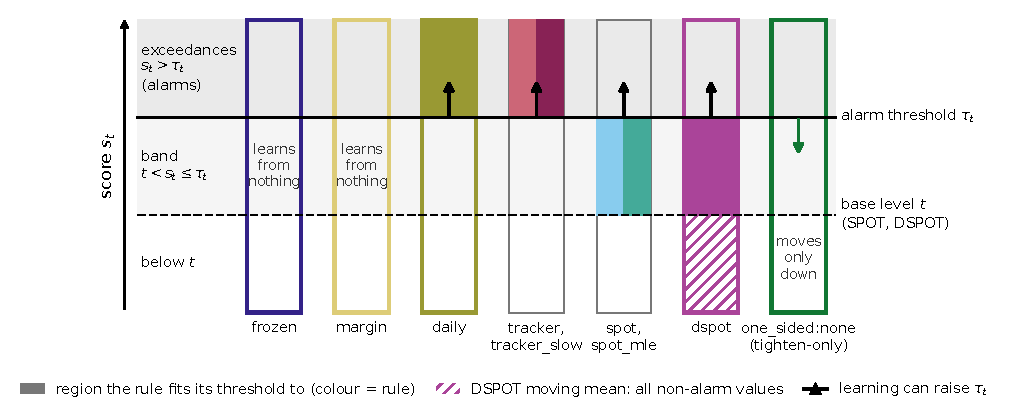
\includegraphics[width=\textwidth]{figures/fig1_learning_regions.pdf}
\caption{Learning regions of the threshold rules (schematic). The alarm threshold $\tau_t$ and, for
SPOT and DSPOT, the base level $t$ below it split the score range into exceedances ($s_t > \tau_t$),
the band ($t < s_t \le \tau_t$) and values below $t$. A filled column segment marks the region a rule
fits its threshold to; DSPOT's moving mean also absorbs every non-alarm value (hatched). Daily
recalibration and the trackers learn from exceedances, so the attacks they are meant to detect raise
their thresholds; frozen and the static margin learn from nothing; one\_sided:none can only move
downward. Data status: schematic with no data, so the registered / exploratory / post-hoc label does
not apply; the rule behaviour follows Table~\ref{tab:regions}.}
\label{fig:regions}
\end{figure*}

A rule can loosen (raise $\tau_t$) only through values in the part of its learning region that
pushes upward. That gives three attacker classes, from weakest to strongest:

\begin{itemize}
\item \textbf{A0, no attacker.} Real attacks are themselves exceedances. A rule whose upward
  learning region includes exceedances is poisoned by the attacks it is meant to detect.
\item \textbf{A1, open-loop injection.} The attacker can perturb one control loop (setpoints or
  sensor readings) without seeing the monitor. Supra-threshold pulses land in the exceedance
  region; sub-alarm pulses land in the band.
\item \textbf{A2, closed-loop.} The stealthy attacker of control
  security~\cite{cardenas2011process, urbina2016stealthy}, turned against an adaptive threshold: it can
  read $\tau_t$ (white-box, or by probing) and shape the score. Holding $s_t$ at $0.97\,\tau_t$ places
  every sample at the top of the band with no
  alarm. We evaluate A2 at the score level, an upper bound on what a physical attacker can do, and
  through noise spoofed onto three sensor readings of one loop, scored by the real monitor.
\end{itemize}

The attacker's goal is a terminal attack that the frozen threshold would detect but the adapted
threshold does not.

\paragraph{Why poison rather than conceal}
An A2 attacker who can spoof sensors could also try to hide the terminal attack directly, by spoofing
the readings it disturbs. Poisoning moves that work earlier: after the campaign the terminal step runs
unmodified, so the attacker does not have to keep every reading it changes consistent with normal
operation, which constrained-concealment attacks must do~\cite{erba2020concealment}. We did not compare
the two strategies. The A1 assumption that operators acknowledge recurring alarms without
investigating is the condition alarm-management standards try to remove~\cite{isa182}; our pulse
campaign adds twelve pulses a day, and the frozen threshold alarmed on 92\% of them on
HAI 20.07 (registered E4).

\subsection{How long a threshold remembers}
\label{sec:memory}

Three facts follow from the update rules alone. They predict most of what
Sections~\ref{sec:registered} and~\ref{sec:regions} measure. Proposition~1 restates, as a
memory, the counting identity behind the long-run coverage guarantee of adaptive conformal
inference~\cite{gibbs2021aci}, from which Atarmla~\cite{atarmla2026price} derives the excess alarms a
persistent step produces before the tracker absorbs it. What we add is its reading in terms of the
calibrated false-alarm rate and its check on recorded attacks.

\paragraph{Proposition 1 (tracker memory)} \emph{Under $q_{t+1} = q_t + \eta(\mathbf{1}[s_t > q_t]
- p)$, each step with $s_t > q_t$ raises the threshold by $\eta(1-p)$ and each other step lowers it
by $\eta p$. A rise built from $E$ exceedance steps therefore takes $E(1-p)/p$ quiet steps to undo,
whatever the step size $\eta$.}

The calibrated exceedance rate $p$ sets the memory. On HAI 20.07 ($p = 7.2 \times 10^{-4}$ per
second) the ratio is 1,385, so one minute above the threshold keeps it raised for 23 hours. On
BATADAL ($p = 0.0075$ per 15-minute step) it is 133, so one step above the threshold keeps it raised
for 33 hours. The step size sets how high an exceedance lifts the tracker, not how long the lift
lasts: on BATADAL, where $\eta$ is $6.9\,\tau_0$ per step, one exceedance step lifts it by almost seven
times $\tau_0$. A slower tracker (tracker\_slow, $\eta/10$) climbs less during a short attack but needs
the same 1,385 quiet seconds per exceedance second to come back down, which is why it lost recall too
(Section~\ref{sec:inflate}). Recovery time bounds blind time from above: the tracker misses a later
attack only while it sits above that attack's score. Post-hoc checks on the recorded trajectories
agree with the proposition: every change of the tracker on the HAI 20.07 and BATADAL test streams is
a whole number of these up and down steps (largest deviation $7 \times 10^{-6}$ of a step), and from its final levels the tracker would have needed 43 to 209 days of exceedance-free data to return
to $\tau_0$.

\paragraph{Proposition 2 (daily memory)} \emph{Daily recalibration sets the next day's threshold to
the $(1-p)$ quantile of the last day's $N$ steps. An attack that holds the score above a level $a$
for more than $pN + 1$ steps of one day lifts the next day's threshold to at least $a$.}

That is 64 seconds on HAI 20.07 and two 15-minute steps on BATADAL. The memory is one day, so daily
recalibration is poisoned whenever attacks fall on consecutive days, as they do in the HAI test
files, and it still catches an attack whose first day follows a quiet one. On BATADAL, whose attacks
last one to five days and begin 1.7 to 24 days after the previous one ends (post-hoc, from the recorded
labels), it caught 14 of 14 with its threshold at $0.69\,\tau_0$ at the median onset (registered tt1b).

\paragraph{Proposition 3 (tighten-only)} \emph{If $\tau_t \le \tau_0$ at every step (tighten-only
without a loosening permit), every sample that alarms under the frozen threshold also alarms under
$\tau_t$. The rule therefore detects every event the frozen threshold detects when any alarm inside the
event counts, on any input and against any attacker, adaptive ones included. What it can lose is false
alarms. Under the stricter onset count of Section~\ref{sec:inflate} the guarantee need not hold,
because a lower threshold can start an alarm episode before an attack begins.}

\paragraph{Proposition 4 (ceiling)} \emph{If $\tau_t \le \kappa\tau_0$ at every step, every sample above
$\kappa\tau_0$ alarms, so under the any-alarm count the rule detects every event that the static
threshold $\kappa\tau_0$ detects, on any input and against any attacker.} Proposition~3 is the case
$\kappa = 1$. A ceiling bounds poisoning: whatever the stream held before, an attacker can hide only
events whose score never exceeds $\kappa\tau_0$.

Proposition~3 means the tighten-only results below measure its cost, not its recall. On HAI 20.07,
HyGrid-ICS and voraus-AD its recall and false alarms equalled the frozen threshold's: the inflated
tracker under the cap kept it at $\tau_0$ (post-hoc: on HAI 20.07 it sat below $\tau_0$ in 0.4\% of
minutes). Its own behaviour shows on BATADAL, where the tracker sat below $\tau_0$ for 3.2\% of the
test time (post-hoc) and the rule ran at 2.43 times the false-alarm budget against 0.70 for frozen
(registered), and on a development split of HAI 23.05 (5.98 against 4.05, exploratory). A loosening
permit breaks the guarantee, even one that only an operator could grant: with the registered oracle
permit, a statistical permit that a simulated operator blocks whenever the review window holds a
labelled event, the rule caught the terminal step in 1 of 10 control placements on HAI 20.07, against
10 of 10 for frozen.

\section{Monitor, rules and data}
\label{sec:setup}

\paragraph{Monitor}
D1 is the world-model residual monitor of earlier registered studies on HAI [anonymized]: an
action-conditioned ridge regression with LightGBM residual corrections (60 trees, history 3)
predicts each sensor one and five steps ahead; the score is the mean of the three largest
standardised absolute residuals at each horizon, summed and smoothed over 60\,s. D0 is a model-free
control: the mean of the three largest standardised first differences. Both are calibrated on the
most recent 20\% of normal training data: to 2 false-alarm episodes per day on the 1\,Hz stream
datasets (episodes merged across 60\,s gaps), to a per-sample false-alarm target of 0.05 on
voraus-AD, and to one false-alarm episode per week on BATADAL (episodes merged across 1\,h). In tt1d
one monitor is fitted per operating mode of Tennessee Eastman, calibrated on four of that mode's eleven
development runs, and one for ProvICS; every duration is converted to the dataset's step; and a third
score is a registered secondary: D2, the mean of the three largest standardised residuals after
projection on the principal components that explain 95\% of the variance.

\paragraph{Rules}
frozen ($\tau_0$ at the budget); margin ($\tau_0 + 0.25 \times$ the spread between the calibration
99.9th percentile and median); daily (trailing-day quantile at the calibration exceedance rate $p$);
tracker ($\eta = 0.01 \times$ spread on the stream datasets, $0.05 \times$ spread on voraus-AD) and
tracker\_slow ($\eta / 10$, the best false-alarm adherence among trackers in development);
tighten-only with four automatic permits and an oracle permit that simulates an operator who refuses
to loosen while an event is under way: eleven rules in all. On voraus-AD the spread is the
calibration 99th percentile minus the median and daily recalibration happens every 50 samples. The
streaming extreme-value rules (SPOT and DSPOT, with method-of-moments and maximum-likelihood tail
fits~\cite{hosking1987gpd, siffer2017spot}) were not part of the tt1 registration: they enter in
Section~\ref{sec:regions} as exploratory and post-hoc analyses and are registered in the BATADAL
replication (tt1b) and, in their standard maximum-likelihood form, in tt1d.

\begin{table*}[t]
\caption{Datasets. Event counts are the labelled events of each final split.}
\label{tab:data}
\begin{tabularx}{\textwidth}{@{}LLLLL@{}}
\toprule
Dataset & System & Training data & Final data & Events \\
\midrule
HAI 20.07 (primary) & HIL testbed (boiler, turbine, water treatment) & 547,624\,s normal, 31 sensors, 20 actions & test1 + test2, 5.15 days & 38 attacks \\
HyGrid-ICS & simulated hybrid grid SCADA, 5\,Hz to 1\,Hz & 9.6\,h (label-blind first 40\%) & 14.5\,h & 91 attacks \\
voraus-AD & industrial robot, 100\,Hz to 10\,Hz & 948 normal samples & 1174 samples & 755 anomalous samples \\
HAI 21.03, 22.04, 23.05 (development) & HIL testbed & normal training data & spent test files & 50, 58, 52 attacks \\
BATADAL (registered replication) & water distribution network, 15\,min & 384 days normal & two test files, 260 days & 14 attacks \\
Tennessee Eastman (tt1d) & simulated chemical process, 7 modes, 3.6\,s & 11 attack-free runs of 120\,h per mode & 142 attack runs; 56 sealed attack-free runs & 245 attacks \\
ProvICS (tt1d) & reactor twin under a real PLC, 2\,s & 39\,h attack-free & 21\,h attack recording; 13\,h sealed attack-free & 32 events \\
\bottomrule
\end{tabularx}
\end{table*}

\paragraph{Registration}
The protocol fixed the monitor, splits, rules, injection designs, gates and seeds; the harness
recorded one ledger entry per dataset before reading a test array, refused to run if a frozen file's
SHA-256 differed from the registration, and computed the gates from its own output. A verifier
checks that each access followed the registration commit, that the ledger holds no access the
protocol does not allow, and that the stored gates match a recomputation (27 of 27 checks pass for
tt1, 8 of 8 for tt1b, and 17 of 17 and 20 of 20 for the two datasets of tt1d). tt1d keeps two ledger
entries per dataset, for its attack data and its sealed attack-free data; ProvICS has three of each: a
failed first attempt, a count of missing values, and the amended attempt (Section~\ref{sec:provics}).

\paragraph{Development}
The registered claim of tt1 differs from the one we set out to test. We began with a tighten-only
threshold that loosens through a statistical permit, moved to a static safety margin, and registered
frozen against adaptive after the first two lost recall or missed the budget on the development
releases (Appendix~\ref{sec:development}).

\section{Registered results}
\label{sec:registered}

\subsection{Primary: HAI 20.07}

\begin{table*}[t]
\caption{Registered gates of tt1 on HAI 20.07. Data status: \textbf{registered}.}
\label{tab:gates}
\begin{tabular}{@{}p{0.05\textwidth}p{0.54\textwidth}p{0.33\textwidth}@{}}
\toprule
Gate & Registered test & Result \\
\midrule
G1 & after a pulse campaign ($12 \times 120$\,s per day at twice the terminal magnitude), daily, tracker and tracker\_slow detect the terminal step in at most (frozen $-$ 0.5) of placements; frozen at least 0.8 & frozen 10/10, each adaptive rule 0/10: pass, but uninformative (the adaptive controls were already 0/10) \\
G2 & recall(tracker) $-$ recall(frozen) on the real attacks, 95\% paired event bootstrap upper bound below 0 & 0.526 vs 0.947, $-0.42$ $[-0.58, -0.26]$: pass \\
G3 & frozen false-alarm episodes per day on unlabelled test time at most 4 & 2.23: pass (above the 2.0 budget; in alarm for 39\% of the unlabelled time, post-hoc) \\
\bottomrule
\end{tabular}
\end{table*}

False-alarm episodes per day are counted over the 4.94 days of unlabelled time inside the 5.15-day
test streams. G1 passes as registered, but on this stream the pulses were not needed: the adaptive
rules also missed the terminal step in the control runs, because the test stream's real attacks had
already raised their thresholds 7 to 26 times above $\tau_0$. The pulse effect in isolation comes
from development on attack-free normal data (frozen 30/30; daily 4/30, control 21/30; tracker 1/30,
control 23/30; tracker\_slow 3/30, control 25/30). Neither registered test of a deliberate campaign, G1
here or H3 on BATADAL (Section~\ref{sec:batadal}), could show an effect, because the rules under test
were already blind in the controls; the campaign results in Section~\ref{sec:regions} are exploratory, and those of
Section~\ref{sec:tepcampaigns} registered.

\subsection{Real attacks inflate adaptive thresholds}
\label{sec:inflate}

\begin{table*}[t]
\caption{Event recall and the paired difference against the frozen threshold (95\% paired event
bootstrap) on the D1 score. Data status: \textbf{registered} (tt1).}
\label{tab:recall}
\begin{tabularx}{\textwidth}{@{}Lccccc@{}}
\toprule
Dataset (events) & frozen & daily & tracker & tracker\_slow & tighten-only \\
\midrule
HAI 20.07 (38 attacks) & 0.947 & 0.474 $[-0.63, -0.32]$ & 0.526 $[-0.58, -0.26]$ & 0.711 $[-0.37, -0.11]$ & 0.947 \\
HyGrid-ICS (91 attacks) & 0.297 & 0.297 & 0.154 $[-0.22, -0.08]$ & 0.165 $[-0.21, -0.07]$ & 0.297 \\
voraus-AD (755 anomalous samples) & 0.334 & 0.148 $[-0.21, -0.16]$ & 0.082 $[-0.28, -0.22]$ & 0.213 $[-0.14, -0.10]$ & 0.334 \\
\bottomrule
\end{tabularx}
\end{table*}

At HAI 20.07 attack onsets the median threshold stood at 25.6 $\tau_0$ for daily recalibration, 12.9
for the tracker and 6.4 for the slow tracker. HyGrid's daily rule equals frozen because its 14.5\,h
final never completes a day.

On HAI 20.07 and BATADAL every disagreement between an adaptive rule and the frozen threshold went one way. On HAI 20.07 the
frozen threshold caught 16 attacks the tracker missed and the tracker caught none that it missed
(exact McNemar $p = 3.1 \times 10^{-5}$); the slow tracker split 9 to 0 ($p = 0.0039$) and daily
recalibration 18 to 0 ($p = 7.6 \times 10^{-6}$). On BATADAL the tracker split 8 to 0 ($p = 0.0078$).
These counts are post-hoc, from the recorded trajectories, which reproduce every registered event
count.

\paragraph{Time in alarm and onset recall (post-hoc)}
Episode counts hide how long an alarm lasts. On HAI 20.07 the frozen threshold was in alarm for 39\%
of the unlabelled time. The D1 score sat above $\tau_0$ for the first 23.8\,h of test1, of which the
first 2.7\,h carry no attack label and seven attacks begin inside the rest, and for a 17-hour stretch of test2 that opens with an attack and holds two more. An alarm episode that overlaps an attack does not count as a false
alarm, so the registered episode count records none of these hours. Ten of the frozen threshold's 36
detections were attacks that began while an alarm was already running, nine of them inside these two runs. Counting an attack
only when an alarm episode starts inside it, the detection rule that the authors of the Sherlock
dataset recommend~\cite{wagner2025sherlock}, the frozen threshold detects 26 of 38, the tracker 20
($-0.16$, $[-0.37, 0.05]$), the slow tracker 27 ($+0.03$, $[-0.18, 0.24]$) and daily recalibration 11 ($-0.39$, $[-0.55, -0.24]$). On BATADAL the frozen threshold was in alarm for 1.4\% of the unlabelled
time and the stricter count changes nothing (tracker $-0.57$, $[-0.79, -0.29]$). On HyGrid-ICS (4.1\%
in alarm) the 91 attacks cover 83\% of the final rows, about 100\,s apart on average, so one merged
alarm episode spans several attacks and the stricter count credits few of them: frozen 3 of 91,
tracker 8 ($+0.05$, $[0.00, 0.11]$), slow tracker 5. There the stricter count reverses the sign, but
it measures how alarms merge across back-to-back attacks more than what the threshold detects. G2
stands as registered, but the tracker's HAI 20.07 gap depends on crediting the frozen threshold's long
alarms; the BATADAL gap does not. An earlier post-hoc variant hid each file's opening run above
$\tau_0$ from the threshold update and gave tracker $-0.29$ $[-0.45, -0.16]$ and slow tracker $-0.08$
$[-0.18, 0.00]$; we superseded it because the opening run of test1 turned out to contain seven
attacks.

\begin{figure}[t]
\centering
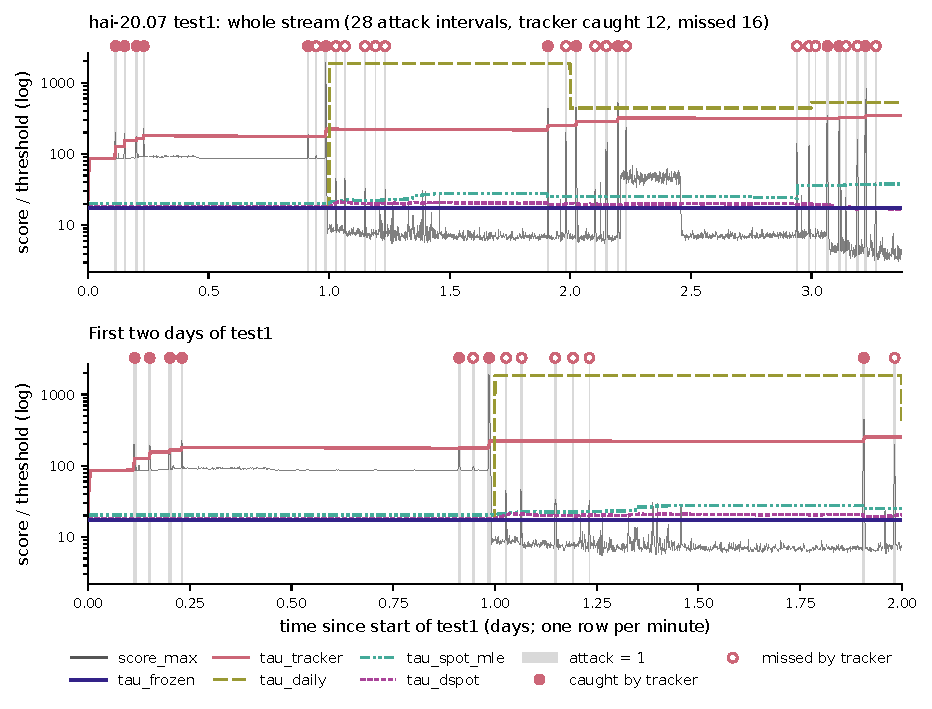
\includegraphics[width=\columnwidth]{figures/fig2_trajectories_hai2007.pdf}
\caption{Threshold trajectories on the HAI 20.07 test1 stream (4,860 minutes). Grey: the D1 score
score\_max. Coloured: the frozen, tracker, daily, spot\_mle and dspot thresholds, log scale. Grey
shading marks attack-labelled minutes; each marker above the panel is one attack interval, filled if
the tracker caught it. test1 holds 28 of the 38 attacks; the tracker caught 12. The score stays above
$\tau_0 = 17.26$ for the first 23.8\,h of test1, so the frozen threshold is in alarm throughout; only
the first 2.7\,h carry no attack label, and seven attacks begin inside the run. That unlabelled opening
lifted the tracker to $5.0\,\tau_0$ before the first attack ($5.25\,\tau_0$ at its onset), and the early
attacks then raised the tracker and daily thresholds far above frozen. Later attacks arrive under the
inflated thresholds. Data status: \textbf{post-hoc analysis}; the trajectories were computed
after the registered finals. The recomputed calibration threshold equals the registered one exactly.
Over test1 and test2 the traces give frozen 36/38 and tracker 20/38 (registered tt1) and spot\_mle
35/38 and dspot 36/38 (post-hoc: SPOT and DSPOT were not in the tt1 registration). test2 is not
drawn; test1 has no missing values.}
\label{fig:hai}
\end{figure}


\subsection{False alarms}

\begin{table}[t]
\caption{False alarms. Data status: \textbf{registered} (tt1).}
\label{tab:falsealarms}
\small
\begin{tabularx}{\columnwidth}{@{}Lccccc@{}}
\toprule
Dataset & frozen & margin & daily & tracker & tracker\_slow \\
\midrule
HAI 20.07 (episodes/day) & 2.23 & 2.23 & 0.20 & 1.01 & 2.23 \\
HyGrid-ICS (episodes/day, 2.5\,h unlabelled) & 19.2 & 0.0 & 19.2 & 19.2 & 19.2 \\
voraus-AD (per-sample FPR, target 0.05) & 0.081 & 0.033 & 0.086 & 0.012 & 0.014 \\
\bottomrule
\end{tabularx}
\end{table}

Where an adaptive rule raised fewer false alarms than frozen, it bought them with the recall losses of Section~\ref{sec:inflate}, except for the oracle permit on voraus-AD (0.064 against 0.081 at equal recall), which uses the attack labels. The one rule that cut false alarms at no recall cost here, the static
margin on HyGrid-ICS (0.0 against 19.2 per day at identical recall), does not adapt. The margin
matched frozen recall on HAI 20.07 and held voraus-AD's target at a cost of 12 points of recall
there. Counted in time rather than episodes (post-hoc), the frozen threshold was in alarm for 39\% of
the unlabelled time on HAI 20.07, 4.1\% on HyGrid-ICS and 1.4\% on BATADAL; the tracker for 0.2\%, 0.3\%
and 0.4\%. Tighten-only equalled the frozen threshold on all three tt1 datasets (2.23, 19.2 and 0.081).

\subsection{Other registered outcomes}
\label{sec:other}

The protocol commits us to report every rule, gate and failure; Appendix~\ref{app:other} gives the rest
of the registered record. Every automatic loosening permit lost recall on HAI 20.07, and the oracle
permit, which equalled frozen on the real attacks, caught the terminal step in 1 of 10 control
placements of the G1 campaign.

\section{Registered replications}
\label{sec:replications}

\subsection{BATADAL (tt1b)}
\label{sec:batadal}

We registered a second study (tt1b) to test the exploratory findings of Sections~\ref{sec:evt}
and~\ref{sec:frog} on data no analysis here had opened: the C-Town network of
BATADAL~\cite{taormina2018batadal}, whose original attacks conceal themselves in the SCADA readings,
in the re-simulation without that concealment published with the artifact of Erba
et al.~\cite{erba2020concealment}, put on a 15-minute grid. All time-scale settings were fixed in
physical time before access: 1\,h smoothing, episodes merged across 1\,h, one false-alarm episode per
week, a one-day DSPOT mean. The test files hold 14 attacks in 260 days.

\begin{table*}[t]
\caption{Registered hypotheses of tt1b on BATADAL. Data status: \textbf{registered}.}
\label{tab:tt1b}
\begin{tabular}{@{}p{0.10\textwidth}p{0.46\textwidth}p{0.36\textwidth}@{}}
\toprule
Hypothesis & Registered test & Result \\
\midrule
H1 & recall(tracker) $-$ recall(frozen), interval upper bound below 0 & 6/14 vs 14/14, $-0.57$ $[-0.79, -0.29]$: pass \\
H2 & recall(MLE SPOT) $-$ recall(frozen), lower bound at least $-\max(0.10, 2/N)$ & 14/14, difference 0: pass \\
H3 & 24\,h closed-loop frog: DSPOT at least 0.5 below its control; frozen and tighten-only within 0.1 & DSPOT already 0/10 in the control: fail \\
Primary rule & H1 and H2 and H3 & fail \\
\bottomrule
\end{tabular}
\end{table*}

We retain the primary rule as registered and report H3 as uninformative rather than refuted. H2
passes under the registered bootstrap, whose interval is $[0, 0]$ because no event was discordant; an
exact one-sided 97.5\% bound for 0 discordant events in 14 is $-0.23$, beyond the $-0.14$ tolerance,
so H2 is not informative under an exact method. SWaT and WADI are registered under the same protocol.
We requested them from their publisher on 2026-10-23 and had not been granted access when we
submitted, so the registered replication rests on BATADAL alone; if access arrives, they will run once
under the registration and be reported whatever they show.

H3 could not be tested because DSPOT's control was already blind, and the blindness predates the
attacks. Fitted by the method of moments to BATADAL's heavy-tailed calibration scores (spread 6,462
against $\tau_0 = 9.39$), SPOT's alarm level started at $49.0\,\tau_0$ and DSPOT's at $45.8\,\tau_0$ at
the first step of each test file, and both fell through the streams, to 24 to 44 $\tau_0$ at the first
attack (post-hoc trajectories; the registered per-event onset inflation agrees). Rerun with no attack
sample in their update, SPOT still caught 6 of 14 and DSPOT 7 of 14 (post-hoc). MLE SPOT started at
$1.22\,\tau_0$ and caught all 14. On BATADAL the moments-based extreme-value rules started too high because of their calibration fit; the attacks did not raise them.

The registered frog variants (10 placements each) did test MLE SPOT. Under the 24\,h closed-loop frog
it caught the terminal attack in 7 of 10 placements against 9 of 10 in its control with D1, and in 0 of
10 against 4 of 10 with D0; with 6\,h and 1\,h campaigns it matched its D1 control and caught 2 and 4 of
10 against 4 with D0. Frozen and tighten-only caught 10 of 10 in every variant, daily recalibration 9
of 10, the margin none, and the tracker, SPOT and DSPOT at most 1 of 10 with or without a campaign.
The frozen threshold detected the 14 real attacks a median 3.5 steps (52.5 minutes) after onset and at
most 65 steps (16.3\,h) after.

\begin{table}[t]
\caption{BATADAL, D1 score. Data status: \textbf{registered} (tt1b).}
\label{tab:batadal}
\begin{tabularx}{\columnwidth}{@{}lCCC@{}}
\toprule
Rule (D1) & Recall & False alarms ($\times$ budget) & Onset inflation \\
\midrule
frozen & 14/14 & 0.70 & 1.0 \\
tighten-only & 14/14 & 2.43 & 1.0 \\
SPOT (MLE) & 14/14 & 0.81 & 1.0 \\
daily & 14/14 & 6.34 & 0.69 \\
tracker & 6/14 & 1.83 & 409 \\
tracker\_slow & 5/14 & 0.70 & 74 \\
SPOT (moments) & 6/14 & 0.13 & 26 \\
DSPOT & 6/14 & 0.13 & 24 \\
margin & 3/14 & 0.05 & 173 \\
\bottomrule
\end{tabularx}
\end{table}

\begin{figure}[t]
\centering
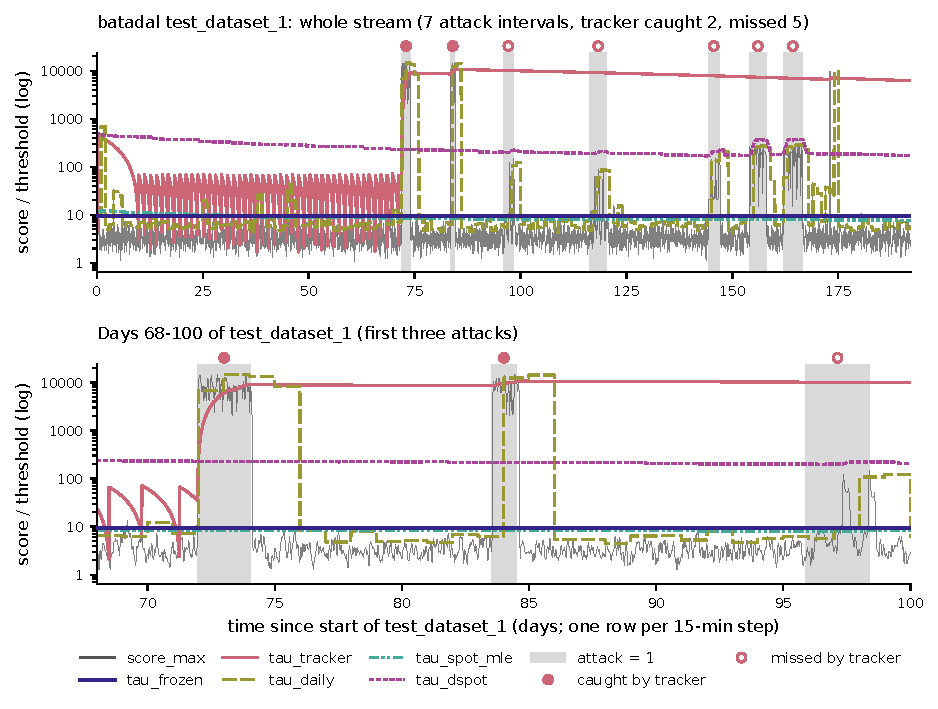
\includegraphics[width=\columnwidth]{figures/fig3_trajectories_batadal.pdf}
\caption{Threshold trajectories on the BATADAL test\_dataset\_1 stream (18,433 steps of 15 minutes,
192 days); layout as in Figure~\ref{fig:hai}. test\_dataset\_1 holds 7 of the 14 attacks; the tracker
caught 2. The lower panel zooms to days 68 to 100, which cover the first three attacks, because the
first attack starts on day 72. score\_max is missing for the first 10 steps ($t = 0$ to 9, 2.5\,h);
those steps are left as a gap and the thresholds are drawn there as given. The attacks lift the
tracker to about $10^4$. DSPOT's moments fit starts $45.8\,\tau_0$ above $\tau_0$ (9.39) at $t = 0$,
before any attack, and falls through the stream, while frozen and spot\_mle stay near $\tau_0$. Data status: \textbf{post-hoc analysis} of the tt1b dataset, which was
opened once for the registered study; the recomputed $\tau_0$ equals the registered value exactly.
Over both test files the traces give frozen 14/14, tracker 6/14, spot\_mle 14/14 and dspot 6/14, the
registered tt1b counts. test\_dataset\_2 is not drawn.}
\label{fig:batadal}
\end{figure}

With the model-free D0 score, MLE SPOT also lost recall (9/14, $[-0.64, -0.14]$). The margin and the
tracker step are scaled by the calibration spread (99.9th percentile minus median); BATADAL's
residual scores are heavy-tailed, so the margin sat 173 times above $\tau_0$. Parameters scaled by a
tail spread are fragile when the tail is heavy.


\subsection{Tennessee Eastman: attacks that follow attacks (tt1d)}
\label{sec:tep}

A third study registered what the first two left open: both detection counts, the mechanism, the
stronger rules and ceilings of Sections~\ref{sec:stronger} and~\ref{sec:bounded}, and campaigns whose
controls can pass or fail. Its main dataset is Kaspersky's Tennessee Eastman attack
set~\cite{filonov2017tep, downs1993tep}: 142 attack runs in seven operating modes and attack-free runs
of 120\,h, one row every 3.6\,s. File names fixed each run's role before any content was read. Per
mode, eleven attack-free runs fit and calibrate one monitor and eight more stayed sealed. Two attack
types hold one attack per run and two hold several in a row: three and four in the dataset's
description, two or three events here, because back-to-back attacks with the same indicators merge
under our event definition. An event is either the \emph{first} of its run (141 events) or a
\emph{follower} (104), and every follower begins within one step of the end of the attack before it.

\begin{table}[t]
\caption{Tennessee Eastman, D1: events detected, and false-alarm episodes over the budget on the 56
sealed attack-free runs (280 days). Data status: \textbf{registered} (tt1d).}
\label{tab:tep}
\small
\begin{tabular}{@{}lrrrr@{}}
\toprule
 & First & \multicolumn{2}{c}{Followers (104)} & False \\
Rule & (141) & any alarm & onset & alarms \\
\midrule
frozen & 116 & 104 & 44 & 0.98 \\
tracker & 116 & 66 & 37 & 1.21 \\
tracker, $\eta = 0.01\,\tau_0$ & 123 & 55 & 37 & 1.64 \\
tracker\_slow & 110 & 88 & 50 & 0.83 \\
daily & 106 & 59 & 40 & 1.22 \\
daily, episodes left out & 113 & 104 & 44 & 1.33 \\
tracker, capped rise & 130 & 104 & 44 & 2.12 \\
tracker, ceiling $1.25\,\tau_0$ & 121 & 104 & 41 & 1.30 \\
SPOT (ML) & 106 & 104 & 43 & 0.84 \\
tighten-only & 122 & 104 & 44 & 1.57 \\
\bottomrule
\end{tabular}
\end{table}

\emph{H1a passed.} The tracker caught 66 of the 104 followers against 104 for the frozen threshold
($-0.37$, $[-0.47, -0.27]$, whole runs resampled; all 38 discordant events favour frozen), and daily
recalibration 59 ($[-0.55, -0.32]$). \emph{H1c passed}: on first events the tracker caught 116 against
116 ($[-0.05, +0.05]$; six discordant events each way). The tracker's loss falls on attacks that follow
attacks and not on the first attack of a run, which is the mechanism of Section~\ref{sec:regions}, here
registered, and it sits in the runs of consecutive noise attacks (57 of 95 events against 95). Daily
recalibration also lost first events (106 against 116, $[-0.12, -0.02]$). \emph{H1b failed}: under the
onset count the tracker caught 37 followers against 44 ($-0.07$, $[-0.13, 0.00]$, the upper bound exactly zero), so the
registered primary rule, H1a and H1b, failed. The registration had named the reason in advance: a follower begins
while the alarm of the attack before it is still running, and the onset count then credits the frozen
threshold with only 44 of the 104 followers it alarmed on. \emph{H2 passed}: the excluding
recalibration and the capped tracker each caught all 104 followers. H3, the ceiling's consistency with
Proposition~4, held on every event. With D0 (secondary) the tracker again lost followers and not first
events ($[-0.30, -0.10]$ and $[-0.06, +0.07]$). With D2 it tightened instead: on the
unlabelled time of the attack runs it ran at 33 times the false-alarm budget, against 1.7 for frozen,
and caught 134 first events against 79, with a follower difference of $[-0.11, +0.03]$.
Appendix~\ref{app:tt1d} lists every registered rule.

\subsection{Tennessee Eastman: registered campaigns}
\label{sec:tepcampaigns}

Each of the 56 sealed attack-free runs received one campaign placement, drawn after its first 12\,h: a
24\,h campaign at the score level, one quiet hour, then a 600\,s terminal bump
(Table~\ref{tab:tepcampaigns}). The loud campaign sets the score to $2\,\tau_0$ for 120\,s every 2\,h;
the frog and the sub-event pulses are those of Section~\ref{sec:bounded}, with every duration rounded
to the 3.6\,s step (a sub-event pulse lasts 43\,s).

\begin{table*}[t]
\caption{Campaigns on the 56 sealed attack-free Tennessee Eastman runs: terminal bumps of 1.05 / 1.25 /
1.5\,$\tau_0$ caught after the campaign, of 56. Without a campaign the adaptive rules caught 44 to 51
bumps of $1.05\,\tau_0$ and 55 or 56 of the larger ones; the frozen threshold caught all 56. Data
status: \textbf{registered} (tt1d).}
\label{tab:tepcampaigns}
\begin{tabularx}{\textwidth}{@{}Lccc@{}}
\toprule
Rule & 24\,h frog & Loud pulses & Sub-event pulses \\
\midrule
frozen & 56 / 56 / 56 & 56 / 56 / 56 & 56 / 56 / 56 \\
tracker (as registered in tt1) & -- & 0 / 0 / 0 & 0 / 0 / 0 \\
daily recalibration & -- & 0 / 0 / 0 & 0 / 0 / 0 \\
daily, alarm episodes left out & 47 / 56 / 56 & 49 / 56 / 56 & 0 / 0 / 0 \\
tracker, rise stopped after 60\,s of alarm & -- & 0 / 0 / 0 & 0 / 0 / 0 \\
tracker, rise capped at $0.1\,\tau_0$ per day & 51 / 56 / 56 & 8 / 55 / 56 & 6 / 55 / 56 \\
SPOT, maximum likelihood & 0 / 16 / 24 & 44 / 56 / 56 & 44 / 56 / 56 \\
SPOT, ceiling $1.25\,\tau_0$ & 0 / 16 / 56 & -- & -- \\
tracker, ceiling $1.25\,\tau_0$ & 46 / 56 / 56 & 0 / 56 / 56 & 0 / 56 / 56 \\
daily, ceiling $1.25\,\tau_0$ & -- & 0 / 0 / 56 & 0 / 0 / 56 \\
SPOT, approval every 6\,h / daily & 1 / 17 / 24, \ 32 / 42 / 53 & -- & -- \\
\bottomrule
\end{tabularx}
\end{table*}

All three campaign hypotheses passed. \emph{H4}: after the frog the standard SPOT caught 16 of 56
bumps of $1.25\,\tau_0$ against 56 in its control ($[-0.82, -0.59]$), and with a ceiling at
$1.25\,\tau_0$ all 56 bumps of $1.5\,\tau_0$. In the rehearsal SPOT's own level started up to
$1.06\,\tau_0$, which is why H4 was registered at $1.25\,\tau_0$ and not $1.05\,\tau_0$. \emph{H5}:
after the loud pulses the tracker caught none of 56 bumps of $1.05\,\tau_0$ against 45 in its control,
and the excluding recalibration was unchanged (49 against 49). \emph{H6}: the sub-event pulses left
the excluding recalibration and the hold-off tracker with none of 56, against 49 and 47, while both
ceilings caught all 56 bumps of $1.5\,\tau_0$ (in 4 of the 56 placements an alarm episode of the
excluding rule still reached event length). The frozen threshold caught every bump in every campaign
and control. The quiet-log approval gate (secondary) caught 1 of 56 bumps of $1.05\,\tau_0$ after the
frog with a review every 6\,h and 32 with a daily review, against 44 in its control. Over the 280
sealed attack-free days the frozen threshold ran at 0.98 times its false-alarm budget
(Table~\ref{tab:tep}); the adaptive rules ran above it, from 1.21 for the tracker to 2.12 for the
capped tracker, except SPOT (0.84).

\subsection{ProvICS (tt1d)}
\label{sec:provics}

The second dataset of tt1d is ProvICS~\cite{shibbir2026provics}: a chemical reactor twin under a real
PLC, with 32 labelled events in a 21\,h recording. The last quarter of its attack-free recording was
sealed. The registered run stopped with an error before any result was printed or written, because one
sealed row lacks its setpoint values; a ledgered read then counted missing values and nothing else, and a dated
amendment, committed before the second attempt, repeats the previous value in an empty cell and changes
nothing else.

\emph{P1 failed}: the tracker detected exactly the events the frozen threshold detected, 25 of 32
under the any-alarm count and 4 under the onset count. The monitor did not hold its calibration on
this recording. The frozen threshold was in alarm for 44\% of the unlabelled time, at 33 times its
budget, so most of its detections are events inside standing alarms; the tracker reached the same
recall in alarm for 19\% of the unlabelled time, at 6.5 times the budget. Here adaptation cost no recall and
removed false alarms. P2 and P3 held: the capped tracker and every ceiling rule detected the same 25 events. With D2
(secondary) the tracker lost 9 of the 25 events ($[-0.44, -0.12]$). On
the sealed rows (six overlapping placements of a 6\,h campaign, descriptive) the loud pulses left the
tracker with none of 6 bumps of $1.05\,\tau_0$ and the sub-event pulses left the hold-off tracker with
none of 6, but the frog did not move SPOT, whose level rose by 0.6\% and which caught all 6 (P4 failed).

\section{Learning regions under attack (exploratory)}
\label{sec:regions}

The analyses in this section were not registered. They use the spent HAI releases for development
and reopen the three tt1 datasets after their finals; every access is in the ledger.

\subsection{Extreme-value thresholds escape natural poisoning on the HAI data}
\label{sec:evt}

On the three spent releases the moments SPOT, the maximum-likelihood SPOT and DSPOT stayed within two
events of the frozen threshold on each release (recall 0.58 to 1.00 against 0.60 to 1.00), where the tracker lost 22 to 37 points; post-hoc
on HAI 20.07 they caught 36, 35 and 36 of 38 attacks against 36 (Table~\ref{tab:evt} in
Appendix~\ref{app:dev}).

The exceptions: on HyGrid-ICS the moments SPOT lost 9 points ($[-0.15, -0.03]$); on voraus-AD, 190
calibration samples leave about four tail points above SPOT's base level (the calibration 98th
percentile), and SPOT ran at 32\% false positives against a 5\% target. On the HAI data the
extreme-value thresholds started near calibration: at the start of both HAI 20.07 test files the
moments SPOT stood at $1.09\,\tau_0$, DSPOT at 1.03 to 1.05 and MLE SPOT at 1.18 (post-hoc).
Section~\ref{sec:batadal} shows what a heavier calibration tail does to that starting point.

\subsection{The effect does not depend on the score}

With D0 the tracker lost recall on every dataset where it was measured: $[-0.38, -0.14]$,
$[-0.21, -0.05]$ and $[-0.19, -0.02]$ on the spent releases (exploratory), $[-0.32, -0.08]$ on HAI
20.07, $[-0.12, -0.02]$ on HyGrid-ICS and $[-0.04, -0.01]$ on voraus-AD (post-hoc), and
$[-0.86, -0.36]$ on BATADAL (registered tt1b). With the reconstruction score D2
(exploratory here), the frozen threshold caught 65 of the 160 events of the development releases and
the tracker 53 ($[-0.14, -0.01]$) pooled; on HAI 22.04 the tracker tightened instead and caught 18
against 11, at 31 false alarms a day.

\subsection{Mechanism: attacks that follow attacks}

The tracker's misses concentrate on attacks that start within 6\,h of the previous attack's end. D1
recall on close versus isolated attacks was 0.75 / 1.00, 0.41 / 1.00 and 0.20 / 0.67 on the spent
releases and 0.48 / 0.71 on HAI 20.07 (31 close, 7 isolated). The frozen threshold also detected
close attacks less often on two releases, so part of the gap reflects harder attacks; the tracker's
gap is larger on every release.

Attacks are the main thing that raises the tracker. Rerun post-hoc with its update fed only the
attack-labelled samples (the others replaced by the calibration median for the update, alarms still on
the real score), the tracker detected 20 of 38 on HAI 20.07 and 14 of 91 on HyGrid-ICS, exactly its
registered counts, and 7 of 14 on BATADAL (6 registered). Fed only the unlabelled samples, it detected
28 of 38, 27 of 91 (equal to frozen) and 11 of 14: the unlabelled exceedances add a smaller loss of
their own, $-0.21$ $[-0.34, -0.08]$ on HAI 20.07 and $-0.21$ $[-0.43, 0.00]$ on BATADAL.

\subsection{Loud poisoning: pulse campaigns}
\label{sec:pulses}

Normal data of the spent releases, 30 placements; the terminal step is the smallest setpoint step
the frozen threshold detects on the clean stream. After a campaign of 120\,s supra-threshold pulses, twelve a day for up to a day,
daily recalibration caught 4 of 30 terminal steps (control 21), the tracker 1 (23) and the slow tracker
3 (25); the frozen threshold caught all 30 and SPOT 29 (Table~\ref{tab:pulses} and
Figure~\ref{fig:campaigns} in Appendix~\ref{app:dev}).


Open-loop sub-alarm pulses did not poison SPOT: its threshold fell (0.82 to 0.98 $\tau_0$), and many
pulses crossed SPOT's own alarm level and were refused.


\subsection{Silent poisoning: the closed-loop frog}
\label{sec:frog}

Score-level attacker A2, normal data of the spent releases, 10 placements each: the attacker holds
the score at $0.97\,\tau_t$, then, after a one-hour lead, a 600\,s bump at $1.05\,\tau_0$ follows
(600\,s is the terminal length of every development campaign). After 24\,h the moments SPOT and
DSPOT caught none of 30 terminal bumps and the maximum-likelihood SPOT 8; the frozen threshold, the slow
tracker and tighten-only were unaffected (Table~\ref{tab:frog}).


Each rule is compared with its own control (the same bump without a campaign). The frozen and both
SPOT controls caught 30/30 and DSPOT's 24/30; the tracker and daily controls already missed some
bumps on the drifting releases, and the campaign did not lower them further. After 1\,h the moments
SPOT threshold stood at 1.1 to 4.5 $\tau_0$; after 24\,h it had grown by more than five orders of
magnitude, and the MLE fit left the floating-point range on one release. A synthetic control with a
light tail (the 60-step moving average of $|N(0, 1)|$, five seeds) did not run away: the moments SPOT
threshold stayed at 0.95 to 0.97 $\tau_0$ and caught every terminal bump, and maximum-likelihood SPOT
rose to a median of 1.02 to 1.04 $\tau_0$ (at most 1.06), though it missed the bump on one of the five seeds in the 24\,h,
6\,h and fixed-level variants. The runaway therefore depends on the heavy tail of real residual
scores.

\paragraph{A physically realizable version}
We also gave the attacker only the readings of three sensors coupled to one setpoint channel, spoofed
with zero-mean noise that keeps the D1 score at 0.97 of the rule's threshold for 6\,h
(Appendix~\ref{app:physfrog}). The maximum-likelihood SPOT caught 4 of 12 terminal steps against 12 in
its control and the moments version 6; DSPOT was unchanged (9 against 9). On HAI 22.04 the median
campaign raised no alarm; on HAI 23.05 it was not silent.

\subsection{Stronger baselines and a standard SPOT (exploratory)}
\label{sec:stronger}

The rules above are the plain versions. After the mock review we fixed four stronger adaptive rules and
three SPOT variants in a written plan and ran them on the spent development releases (the plan was
committed before the runs; one rule was corrected by a dated amendment after the first run, and every
run was then repeated). They are daily recalibration that leaves out alarm episodes longer than 60\,s and
the hour after them; the tracker with its upward steps stopped once an alarm has lasted 60\,s and for an
hour after; a tracker whose rise is capped at $0.1\,\tau_0$ per day; Telemanom's dynamic
threshold~\cite{hundman2018telemanom}; SPOT with a maximum-likelihood tail refitted as the peaks grow by
1\%, also with the shape bounded to $|\xi| \le 0.5$ and with runs declustering; and DSPOT on the
maximum-likelihood tail (Table~\ref{tab:stronger} in Appendix~\ref{app:dev}).


Leaving events out of the update, or capping the rise, removed natural poisoning on these releases: the excluding rule matched frozen recall and the capped tracker missed one more event. Stopping the tracker after a minute of alarm did not, because by
Proposition~1 the first minute of each attack still keeps it raised for about a day. The excluding rule
also resisted the pulse campaign, whose 120\,s pulses count as events. An attacker who knows the 60\,s
event length can keep each exceedance shorter; Section~\ref{sec:bounded} runs that attack. The capped tracker lost a little to the pulses, and
its cap bounds how fast it rises, not how far. Telemanom's threshold caught more attacks at 16 to 19 times
the false-alarm budget, so its recall is not comparable with the others.

The standard SPOT did not escape the closed-loop attacker. Refitted by maximum likelihood, with or without
a bounded shape, it missed the terminal step in all 30 placements of the 24\,h campaign, and DSPOT on the
same tail in all 30. Declustering resisted a continuous frog, which forms a single cluster, but an
attacker who leaves the score clean for two minutes after each minute of pushing blinded it on HAI 22.04
(10 of 30 pooled, against a control of 20).

\subsection{Bounded loosening, sub-event pulses and an approval gate (exploratory)}
\label{sec:bounded}

A second written plan, committed before its runs, tested three things on the same releases. \emph{A
ceiling}: the tracker, daily recalibration and the standard SPOT with the deployed threshold clipped at
$\kappa\tau_0$ (Proposition~4). \emph{Sub-event pulses}: a score-level attacker who knows the 60\,s
event length sets the score to twice the current threshold for 45\,s every 30 minutes for a day, so
that a pulse by itself is too short to count as an event. \emph{An approval gate}: SPOT proposes its level, and a
ceiling rises to it at each review if the review window held no alarm, a stand-in for an operator who
signs a loosening when the alarm log is quiet. Campaigns end in terminal bumps of 1.05 to
$10\,\tau_0$ (Table~\ref{tab:bounded}).

\begin{table*}[t]
\caption{Ceilings, sub-event pulses and an approval gate on the three spent HAI releases. Natural
poisoning: events detected of 160. Campaigns: terminal bumps of 1.05 / 1.5 / 3\,$\tau_0$ caught after the
campaign, of 30 placements; where a rule's control at $1.05\,\tau_0$ was below 30 it is given in
parentheses. Data status: \textbf{exploratory}.}
\label{tab:bounded}
\begin{tabularx}{\textwidth}{@{}Lccc@{}}
\toprule
Rule & Natural poisoning & 24\,h frog & Sub-event pulses \\
\midrule
frozen & 125 & 30 / 30 / 30 & 30 / 30 / 30 \\
tracker (as registered) & 77 & -- & 0 / 0 / 0 (20) \\
tracker, ceiling 1.1 / 1.25 / 1.5\,$\tau_0$ & 125 / 118 / 108 & -- & 6 / 30 / 30 (25), \ 0 / 30 / 30 (20), \ 0 / 30 / 30 (20) \\
daily recalibration & 104 & -- & 0 / 5 / 24 (18) \\
daily, ceiling 1.1 / 1.25 / 1.5\,$\tau_0$ & 125 / 121 / 119 & -- & 0 / 30 / 30 (18), \ 0 / 30 / 30 (18), \ 0 / 5 / 30 (18) \\
daily, alarm episodes left out & 125 & 30 / 30 / 30 & 0 / 11 / 30 \\
tracker, rise stopped after 60\,s of alarm & 89 & as control & 0 / 0 / 0 (21) \\
tracker, rise capped at $0.1\,\tau_0$ per day & 124 & 30 / 30 / 30 & 13 / 30 / 30 \\
SPOT, maximum likelihood & 126 & 0 / 0 / 10 & 30 / 30 / 30 \\
SPOT, ceiling 1.1 / 1.25 / 1.5\,$\tau_0$ & 126 / 126 / 126 & 0 / 30 / 30, \ 0 / 30 / 30, \ 0 / 7 / 30 & -- \\
SPOT, approval every 6\,h / daily & 127 / 127 & 15 / 19 / 30, \ 25 / 30 / 30 & -- \\
\bottomrule
\end{tabularx}
\end{table*}

With a ceiling at $1.1\,\tau_0$ the tracker and daily recalibration caught the 125 events the frozen
threshold caught. Wider ceilings cost recall, as Proposition~4 allows: at 1.25 and $1.5\,\tau_0$ the
tracker caught 118 and 108, against 116 and 107 for the static thresholds at those levels. The frog
shows what a ceiling buys. Without one, the standard SPOT missed every terminal bump up to
$1.5\,\tau_0$, and on two of the three releases every bump up to $10\,\tau_0$, because its threshold
left the floating-point range. With a ceiling it missed only bumps at or below the ceiling and caught
all 30 above it.

The sub-event pulses defeated both rules that depend on recognising an event. The excluding
recalibration caught none of 30 terminal bumps up to $1.25\,\tau_0$ (control 30) and the tracker with
a hold-off none at any size up to $10\,\tau_0$, since the pulses were too short to be left out. The capped
tracker missed 17 of 30 at $1.05\,\tau_0$ and none from $1.25\,\tau_0$. SPOT, which does not learn
from alarms, was unaffected. The quiet-log gate did not stop the frog: with a review every 6\,h it
caught 15 of 30 bumps at $1.05\,\tau_0$ and 20 of 30 at $2\,\tau_0$; with a daily review, 25 of 30
at $1.05\,\tau_0$ and all 30 above. A campaign that raises no alarm passes an approval that reads
the alarm log.

\section{Design guidance}
\label{sec:design}

A threshold rule's learning region is its attack surface. Every automatic loosening path of the plain rules could be pushed upward: exceedance tracking and daily recalibration by real attacks (registered) and
by loud pulses (exploratory); tail refitting and moving-mean drift tracking by a closed-loop attacker
(exploratory); the spread and shift permits by pulses and benign drift in development, and on the
registered HAI 20.07 stream all four lost recall (Section~\ref{sec:other}). The rules that held were
the ones that never loosen themselves: frozen, and tighten-only without a permit. An operator-gated
permit is only as good as the operator; our stand-in, which blocked loosening only while a labelled
event was in its review window, caught 1 of 10 terminal steps in the G1 controls. A static margin
never loosens either, but it is not safe by construction: on BATADAL its spread-scaled offset sat 173
times above $\tau_0$ and it caught 3 of 14 attacks, as large a recall loss as any we measured.

Two stronger rules that do loosen themselves, daily recalibration that leaves out alarm episodes and a
tracker with a capped daily rise, came within one event of frozen recall on the development releases
(Section~\ref{sec:stronger}). Each still loosens through what it does not exclude: pulses shorter than its event length blinded
the first, and the second rises by as much as its cap allows each day (Section~\ref{sec:bounded}). Telemanom's threshold avoided the losses only at 16 to 19 times the false-alarm budget.

Parts of this advice are established. Process-alarm standards already route alarm changes through
authorised management of change~\cite{isa182, eemua191}, lowering the threshold has been proposed
against poisoning of retrained ICS detectors~\cite{kravchik2021poisoning}, and a bounded false-positive
rate limits what a poisoner can gain~\cite{kloft2012security}. What we add is the asymmetry for adaptive
thresholds, automatic tightening with gated loosening, and its evaluation against natural, loud and
silent poisoning.

We therefore recommend:

\begin{enumerate}
\item \textbf{Let thresholds tighten automatically, never loosen.} A tracker capped at the calibrated
  threshold cannot lose an event the frozen threshold catches (Proposition~3) and can only add
  sensitivity in quiet periods.
\item \textbf{If a threshold must loosen by itself, give it a ceiling.} Under a ceiling
  $\kappa\tau_0$ no poisoning can hide an event above $\kappa\tau_0$ (Proposition~4). On the
  development releases a ceiling of $1.1\,\tau_0$ cost no recall on the recorded attacks, and in every
  campaign a ceiling hid only bumps at or below it.
\item \textbf{Route loosening beyond the ceiling through an operator} who confirms from the process,
  not from the alarm log, that the plant is in normal operation: a gate that approved whenever the log
  was quiet let the silent campaign through. Treat a request to loosen during or soon after an alarm
  as suspect.
\item \textbf{Recalibrate offline on verified clean data}~\cite{cretu2008sanitizing}, as a
  change-controlled event, when drift raises false alarms. Our frozen thresholds held 0.66 to 1.48
  episodes per day on the three
  development test periods and 2.23 on HAI 20.07 against a budget of 2, but on HAI 20.07 the
  threshold was in alarm for 39\% of the unlabelled time, the kind of drift an offline recalibration
  should catch.
\item \textbf{Watch the threshold.} Log $\tau_t$; a threshold that rises during an incident, or climbs
  steadily without alarms, is itself an indicator.
\item \textbf{Budget alarm time as well as episodes.} On HAI 20.07 a 24-hour alarm that overlapped
  seven attacks did not count against the episode budget at all, and an attack that begins inside a
  running alarm gives the operator nothing new to see.
\end{enumerate}

The cost is false alarms. On BATADAL the tighten-only rule ran at 2.43 times the budget against 0.70
for the frozen threshold, and over 280 attack-free days of Tennessee Eastman at 1.57 against 0.98
(both registered); on a development split of HAI 23.05 at 5.98 against 4.05, where a ten times slower
tracker under the cap brought it to 4.05 (exploratory). A frozen threshold is not always the cheaper
one: on ProvICS it ran at 33 times its budget where the tracker ran at 6.5 with the same recall. A static margin can cut that cost: on the HAI 23.05 development split the margin of our development rounds (half the calibration exceedance rate) ran at 0.58 times the budget. The registered margin ($\tau_0 + 0.25$ times the spread) cost recall on voraus-AD (12 points) and BATADAL (11 of 14 attacks); a margin should not be scaled by a calibration spread that a heavy tail sets.

\section{Limitations}
\label{sec:limitations}

\begin{itemize}
\item Three registered primary rules failed: tt1b's through H3, and both of tt1d's, through the onset
  count on Tennessee Eastman and through P1 on ProvICS. The registered support is the individual
  hypotheses that passed. The tracker's loss survives the onset count on BATADAL only (14 attacks), and
  that count is post-hoc there and on HAI 20.07.
\item HAI 20.07 shares a testbed with the development releases. Tennessee Eastman is a simulated
  process whose attacks are large manipulations, and the registered campaigns are confirmed there
  only; on ProvICS the frog did not move SPOT, and the campaigns on HAI are exploratory.
\item The stronger rules, the standard SPOT, the ceilings and the sub-event pulses were developed on
  HAI and registered on Tennessee Eastman; the registered rules of tt1 are the plain versions.
\item The ProvICS result is registered with one dated amendment after a failed first attempt
  (Section~\ref{sec:provics}).
\item On HAI 20.07 the monitor itself drifted: the frozen threshold was in alarm for 39\% of the
  unlabelled time, which inflates its recall under the any-alarm count (Section~\ref{sec:inflate}).
\item HyGrid-ICS is a single simulated day with 2.5\,h of unlabelled final time; voraus-AD anomalies
  are not attacks. Post-hoc, 0.15\% of HyGrid-ICS's label-blind development rows (251 short runs)
  carry an attack label, against 83\% of its final rows, so its calibration is very slightly
  contaminated.
\item The pulse campaigns and both frogs are synthetic. The score-level frog sets the score directly
  and reads $\tau_t$; the physically realizable version also runs the monitor itself on the spoofed
  history to choose each noise scale. Both are white-box upper bounds.
\item SPOT's behaviour depends on the tail estimator and on the score's tail shape; we report both.
\item Parameters scaled by a calibration spread (the static margin and the tracker step) are fragile
  on heavy-tailed scores: on BATADAL the margin sat 173 times above $\tau_0$ and missed 11 of 14
  attacks.
\item Event recall counts any alarm inside a labelled interval, so it credits an attack that falls
  inside an alarm already running; on HAI 20.07 that gave the frozen threshold 10 of its 36
  detections (Section~\ref{sec:inflate}). We do not model operator response time.
\item Our monitor is one world-model residual, one model-free score and a linear reconstruction
  score (exploratory on HAI, a registered secondary in tt1d); nonlinear autoencoder detectors were
  not tested.
\item We did not test a human operator; the approval gate of Section~\ref{sec:bounded} is an
  automated stand-in. Human-approved suppression of detection rules has been observed to
  accumulate and persist~\cite{dhananjeyan2026ratchet}, so routing loosening through people does not by
  itself stop a threshold from ratcheting upward.
\item No claim of runtime authority, deployment safety or incident prevention follows from these
  results.
\end{itemize}

\FloatBarrier
\section{Conclusion}

On HAI 20.07, BATADAL and Tennessee Eastman (registered), a quantile tracker that learns from
exceedances missed attacks that a frozen threshold caught, and on Tennessee Eastman its misses fell on
attacks that follow attacks and not on the first attack of a run. On BATADAL the loss survives counting only alarms that start inside
an attack; on HAI 20.07 and Tennessee Eastman it does not, because later attacks arrive inside alarms
that are already running, and on ProvICS, where the monitor was in alarm for 44\% of the unlabelled time,
the tracker lost nothing. How long a tracker stays raised follows from its calibrated false-alarm rate
alone, so making it slower does not make it forget faster.

Deliberate poisoning was confirmed on sealed attack-free runs: loud pulses blinded the tracker,
sub-event pulses blinded the recalibration that leaves alarms out, and a closed-loop attacker blinded
a standard SPOT, while the frozen threshold caught every later attack and held its false-alarm budget
over 280 days. On Tennessee Eastman every rule we tested that loosens itself was pushed through the part of
its input it learns from; on ProvICS the frog did not move SPOT. A threshold that only tightens itself keeps the frozen threshold's recall by
construction, and a ceiling confines what any of these attacks can hide to events at or below it.
The price is false alarms: on Tennessee Eastman tighten-only ran at 1.57 times the budget and the
tracker under a ceiling of $1.25\,\tau_0$ at 1.30, against 0.98 for frozen.

\bibliographystyle{ACM-Reference-Format}
\bibliography{refs}

\appendix

\section*{Ethical considerations}

All experiments ran offline on public recordings: HAI 20.07 to 23.05, HyGrid-ICS, voraus-AD, the
BATADAL re-simulation, the Tennessee Eastman attack set and ProvICS, each used under its publisher's
terms. No live plant, testbed, vendor product
or operator was involved, and no human subjects took part. The pulse campaigns and both frog attacks
were injected into recorded normal data or into the score; the physically realizable frog changes
recorded sensor values in software and is scored by our own monitor.

The attacks are not new in kind. Boiling-frog poisoning of self-updating detectors has been public
since 2009~\cite{chantin2009frog, rubinstein2009antidote}, and the threshold rules we attack are
textbook algorithms. What the paper adds for an attacker is the observation that an adaptive
threshold widens the window for a later attack; what it adds for a defender is a rule that closes
that window at a known false-alarm cost. We judged that publishing both helps defenders more than
attackers, because the defence is a configuration change (cap the threshold at its calibrated value)
that any operator of an adaptive threshold can apply today. The released code generates attacks only
against recorded data and a score file; it contains no tooling for reaching a control network.

\section*{Open science}

The three pre-registrations, the data-access ledger, the attack and threshold harnesses, the
registered-gate verifiers and the figure data and plotting code are available in the anonymized
artifact at \url{https://anonymous.4open.science/r/thresholds-that-travel-artifact-579B/}, which also contains the result files behind
every number in this paper and the verifier reports (27 of 27 checks for tt1, 8 of 8 for tt1b, 17 of 17
and 20 of 20 for tt1d).
% The de-anonymized repository and the artifact DOI are added in the camera-ready version.
The raw datasets are not redistributed here and are available from their publishers: HAI from its
dataset repository, BATADAL from Taormina et al.~\cite{taormina2018batadal} and the no-concealment
re-simulation from the artifact of Erba et al.~\cite{erba2020concealment}, voraus-AD from Brockmann
et al.~\cite{brockmann2024voraus}, HyGrid-ICS from its Zenodo record~\cite{yolcu2026hygrid}, the
Tennessee Eastman attack set from Kaspersky~\cite{filonov2017tep} and ProvICS from its
authors~\cite{shibbir2026provics}, under whose terms it is not redistributed.
Reproducing the registered results requires one access to each raw dataset under the access rules
recorded in the ledger. For review, the copy withholds the repository's commit history, which the
verifiers use to check that every access followed its registration, and replaces the project name and
commit hashes; its ANONYMIZATION.md lists each replacement.

\section{Other registered outcomes of tt1}
\label{app:other}

Table~\ref{tab:permits} and the list below complete the registered record of tt1.

\begin{table}[t]
\caption{Tighten-only with a loosening permit on HAI 20.07. Data status: \textbf{registered} (tt1).}
\label{tab:permits}
\begin{tabularx}{\columnwidth}{@{}Lcccc@{}}
\toprule
Permit & Recall & vs frozen (95\%) & FA/day & Permits/wk \\
\midrule
spread, daily review & 26/38 & $[-0.39, -0.13]$ & 1.62 & 2.7 \\
spread, 6\,h review & 28/38 & $[-0.34, -0.08]$ & 2.63 & 4.1 \\
shift, daily review & 32/38 & $[-0.21, -0.03]$ & 1.01 & 4.1 \\
shift, 6\,h review & 31/38 & $[-0.24, -0.03]$ & 2.02 & 12.2 \\
oracle & 36/38 & $[0, 0]$ & 2.23 & 0 \\
\bottomrule
\end{tabularx}
\end{table}

\begin{itemize}
\item \textbf{Automatic permits.} Every automatic loosening permit lost recall on HAI 20.07. On
  voraus-AD all four lost recall too (95\% intervals: spread $[-0.21, -0.15]$ with daily review and
  $[-0.28, -0.21]$ with 6\,h review; shift $[-0.18, -0.13]$ and $[-0.21, -0.15]$); on HyGrid-ICS only
  the 6\,h shift permit did (24 of 91, $[-0.08, 0.00]$).
\item \textbf{Oracle permit.} On the real attacks it equalled frozen, but in the G1 campaign runs it
  caught the terminal step in 7 of 10 placements after the pulses and 1 of 10 in the control.
\item \textbf{First and second half of the HAI 20.07 events.} Recall was 0.947 / 0.947 for frozen,
  0.474 / 0.579 for the tracker, 0.579 / 0.842 for the slow tracker and 0.474 / 0.474 for daily
  recalibration.
\item \textbf{E5, sub-threshold noise campaign.} Only 1 of 13 placements admitted a stealthy noise
  level; 12 had none, so E5 gives no result.
\item \textbf{BATADAL frog variants} are in Section~\ref{sec:batadal}. A separate registration that
  shared the HAI 20.07 and HyGrid-ICS access (detection-v2) is reported on its own.
\end{itemize}

\section{The physically realizable frog}
\label{app:physfrog}

The score-level attacker sets the score directly. We also gave the attacker only the readings of
three sensors coupled to one setpoint channel. Every 5 minutes it reads the rule's threshold and
spoofs the largest zero-mean noise whose D1 score, computed by the real world model on the spoofed
history, stays at 0.97 of that threshold; after 6\,h it stops, and 1\,h later the just-detectable
setpoint step follows. This attacker is white-box: it can run the monitor.

\begin{table}[t]
\caption{The physically realizable frog. Data status: \textbf{exploratory} (normal data of the spent
releases).}
\label{tab:physfrog}
\small
\begin{tabular}{@{}p{0.20\columnwidth}p{0.30\columnwidth}p{0.33\columnwidth}@{}}
\toprule
Rule & Terminal steps caught, after campaign / in control (of 12 placements) & Threshold at the terminal step (median per release) \\
\midrule
frozen & 12 / 12 & 1.0 $\tau_0$ \\
SPOT (MLE) & 4 / 12 & 1.04 to 1.59 $\tau_0$ \\
SPOT (moments) & 6 / 12 & 0.78 to 1.42 $\tau_0$ \\
DSPOT & 9 / 9 & 0.87 to 1.12 $\tau_0$ \\
\bottomrule
\end{tabular}
\end{table}

Controls caught 12 of 12 for frozen and both SPOT variants and 9 of 12 for DSPOT, so the campaign did not change DSPOT's total (per release, campaign against control: 4 against 3, 3 against 4 and 2 against 2). On HAI 22.04 both SPOT variants missed the terminal step on all four placements, and the median campaign raised no alarm. On HAI 23.05 it was not silent: the frozen threshold raised a median of
190 alarm steps during the campaign, and the SPOT variants 154 to 171. The
spoofed noise had a scale of 0.02 to 0.04 robust units against frozen and the SPOT variants, and 0.05
to 0.12 against DSPOT, whose moving mean follows the noise-driven rise, so the attacker's cap rises
with the mean rather than with the tail.

\section{Development experiments in detail}
\label{app:dev}

Tables~\ref{tab:evt} to~\ref{tab:stronger} and Figure~\ref{fig:campaigns} give the per-rule results of
the exploratory experiments of Section~\ref{sec:regions}. Figure~\ref{fig:forest} collects the recall differences of tt1, tt1b and
the development releases with their status.

\begin{table*}[t]
\caption{Event recall of the extreme-value rules. Data status: \textbf{exploratory} on the spent
releases, \textbf{post-hoc} on HAI 20.07.}
\label{tab:evt}
\begin{tabularx}{\textwidth}{@{}Lccccc@{}}
\toprule
Data & frozen & tracker & SPOT (moments) & SPOT (MLE) & DSPOT \\
\midrule
HAI 21.03 / 22.04 / 23.05 & 1.00 / 0.76 / 0.60 & 0.78 / 0.45 / 0.23 & 1.00 / 0.79 / 0.58 & 1.00 / 0.79 / 0.60 & 1.00 / 0.79 / 0.60 \\
HAI 20.07 (post-hoc) & 0.947 & 0.526 & 0.947 & 0.921 $[-0.08, 0.00]$ & 0.947 \\
\bottomrule
\end{tabularx}
\end{table*}

\begin{table*}[t]
\caption{Terminal attacks caught after a pulse campaign (control in parentheses). Data status:
\textbf{exploratory} (normal data of the spent releases).}
\label{tab:pulses}
\begin{tabularx}{\textwidth}{@{}Lcccccc@{}}
\toprule
Campaign & frozen & daily & tracker & tracker\_slow & SPOT & DSPOT \\
\midrule
$12 \times 120$\,s supra-threshold pulses per day & 30/30 (30/30) & 4/30 (21/30) & 1/30 (23/30) & 3/30 (25/30) & 29/30 (30/30) & 23/30 (25/30) \\
$24 \times 300$\,s sub-alarm pulses per day, open loop & 30/30 & 23/30 (23/30) & 19/30 (21/30) & 23/30 & 29/30 & 22/30 (24/30) \\
\bottomrule
\end{tabularx}
\end{table*}

\begin{table*}[t]
\caption{Terminal attacks caught after a closed-loop frog campaign, 30 placements. Data status:
\textbf{exploratory} (normal data of the spent releases).}
\label{tab:frog}
\begin{tabular}{@{}lllll@{}}
\toprule
Rule & 24\,h campaign & 6\,h & 1\,h & open loop, fixed level, 24\,h \\
\midrule
frozen, tracker\_slow, tighten-only & as control & as control & as control & as control \\
tracker & as control & as control & as control & 16/30 (control 20/30) \\
SPOT (moments) & 0/30 & 0/30 & 0/30 & not moved; alarms throughout \\
DSPOT & 0/30 & 0/30 & 0/30 & not moved; alarms throughout \\
SPOT (MLE, refit every 2048 peaks) & 8/30 & 8/30 & 13/30 & 11/30 \\
\bottomrule
\end{tabular}
\end{table*}

\begin{table*}[t]
\caption{Stronger adaptive rules and a standard SPOT on the three spent HAI releases. Natural poisoning:
events detected of 160 and the paired difference against frozen (125 of 160). Pulses and frog: terminal
steps caught after the campaign / in the control, of 30 placements. Data status: \textbf{exploratory}.}
\label{tab:stronger}
\begin{tabularx}{\textwidth}{@{}Lccc@{}}
\toprule
Rule & Natural poisoning & Pulses & 24\,h frog \\
\midrule
tracker (as registered) & 77, $[-0.37, -0.23]$ & 1 / 23 & as control \\
daily recalibration & 104, $[-0.19, -0.08]$ & 4 / 21 & as control \\
daily, alarm episodes left out & 125, $[-0.02, 0.02]$ & 30 / 30 & 30 / 30 \\
tracker, rise stopped after 60\,s of alarm & 89, $[-0.29, -0.16]$ & 2 / 24 & 21 / 21 \\
tracker, rise capped at $0.1\,\tau_0$ per day & 124, $[-0.02, 0.00]$ & 25 / 30 & 30 / 30 \\
Telemanom dynamic threshold (33 to 37 false alarms a day) & 140, $[+0.04, +0.15]$ & 27 / 26 & 28 / 28 \\
SPOT, maximum likelihood & 126, $[-0.01, +0.03]$ & 30 / 30 & 0 / 30 \\
SPOT, maximum likelihood, $|\xi| \le 0.5$ & 127, $[0.00, +0.03]$ & -- & 0 / 30 \\
SPOT, maximum likelihood, declustered & 123, $[-0.04, +0.02]$ & 21 / 24 & 20 / 20 (bursts: 10 / 20) \\
DSPOT, maximum-likelihood tail & 127, $[0.00, +0.03]$ & -- & 0 / 24 \\
\bottomrule
\end{tabularx}
\end{table*}

\begin{figure}[t]
\centering
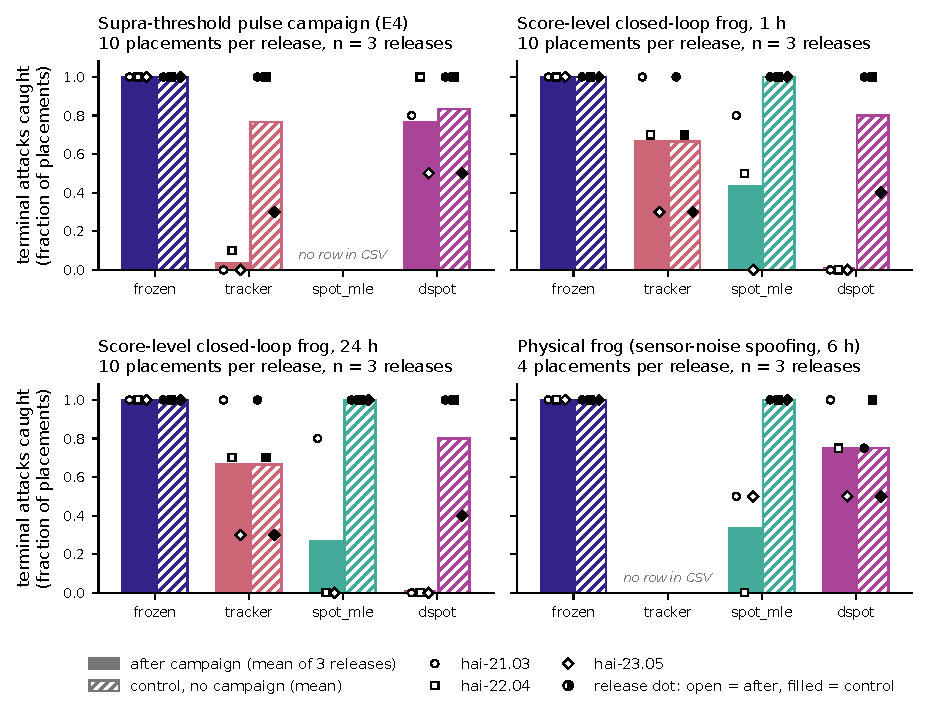
\includegraphics[width=\columnwidth]{figures/fig5_attack_campaigns.pdf}
\caption{Terminal attacks caught after each campaign (solid) and in the matching control (hatched),
for frozen, tracker, spot\_mle and dspot. Each bar is the mean over the three spent HAI releases;
dots are the per-release values, and every release had the same number of placements, so the mean
equals the pooled fraction. Panels: the supra-threshold pulse campaign (E4, 10 placements per
release); the score-level closed-loop frog at 1\,h and 24\,h (10 placements); and the physical frog,
which spoofs noise on three sensors for 6\,h (4 placements). Data status: all four panels are
\textbf{exploratory} results on the normal data of the spent releases. The source CSV has no
spot\_mle row for E4 and no tracker row for the physical frog; both slots are left empty and
labelled.}
\label{fig:campaigns}
\end{figure}

\begin{figure*}[t]
\centering
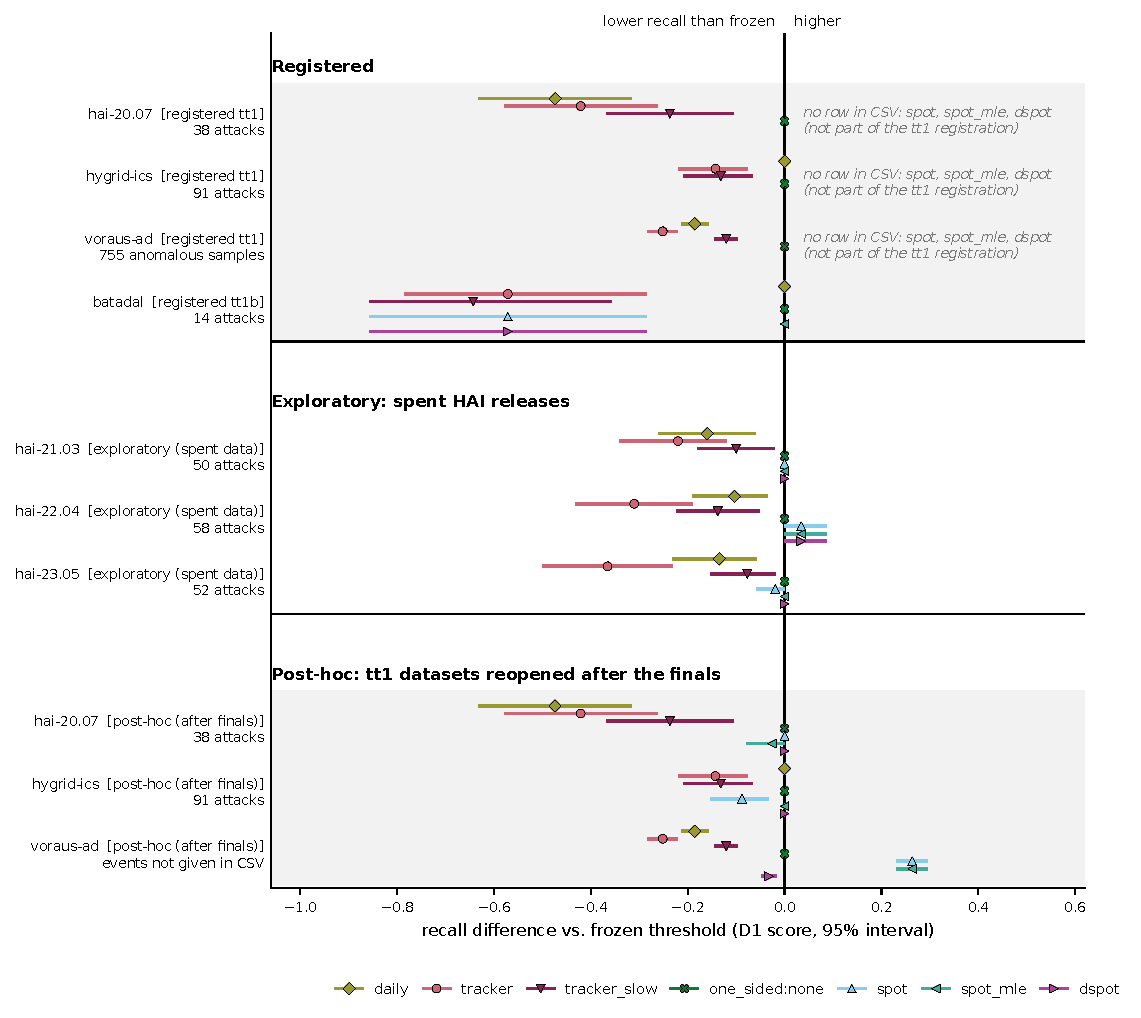
\includegraphics[width=0.92\textwidth]{figures/fig4_recall_forest.pdf}
\caption{Paired difference in event recall between each adaptive rule and the frozen threshold on
D1, with 95\% intervals. Values left of 0 mean lower recall than frozen. Three blocks, each row
labelled with its data status: (1) \textbf{registered} results from tt1 (hai-20.07, hygrid-ics,
voraus-ad) and tt1b (batadal); (2) \textbf{exploratory} development results on the spent HAI
releases; (3) \textbf{post-hoc} results on the tt1 datasets, reopened after the finals. spot,
spot\_mle and dspot have no rows for the registered tt1 datasets because those rules were not part
of the tt1 registration; the gaps are labelled and the post-hoc block supplies the comparisons.
one\_sided:none equals frozen (0 $[0, 0]$) in every block. The positive spot and spot\_mle values
for voraus-ad (post-hoc) are not a gain: with 190 calibration samples SPOT ran at a per-sample
false-positive rate of 0.32 against the 0.05 target (Section~\ref{sec:evt}).}
\label{fig:forest}
\end{figure*}

\FloatBarrier
\section{How the hypothesis changed during development}
\label{sec:development}

All development used normal training data and the already-opened attack files of HAI 21.03, 22.04
and 23.05. We report it because the registered claim differs from the one we set out to test.

\begin{enumerate}
\item \emph{Tighten-only with automatic loosening.} Our starting design let a threshold tighten
  itself and loosen only through a statistical permit. A slow sub-threshold drift (``boiling frog''
  in the style of Rubinstein et al.) did not poison any rule: the world model absorbed the drift.
  Supra-threshold pulses did inflate the trackers, but every automatic permit we tried either opened
  under the pulses (spread permit: 3 of 30 terminal attacks caught in development round r3, 5 of 30
  in round r4) or failed to follow benign drift (shift permit).
\item \emph{Static safety margin.} A margin at half the calibration exceedance rate cut the
  false-alarm rate on pseudo-deployment splits without always reaching the budget (HAI 20.07
  development: 3.79 episodes per day against 4.42 for frozen, budget 2), and cost 4 to 10 points of
  recall on the spent attacks (interval lower bounds down to $-0.17$), so we registered a smaller
  margin and made it secondary.
\item \emph{Frozen versus adaptive.} On the spent attacks the frozen threshold held the budget on
  all three real test periods (0.66, 1.48 and 1.27 episodes per day), while the tracker lost 22, 31
  and 37 points of recall with intervals entirely below zero. This became the registered primary.
\end{enumerate}

\FloatBarrier
\section{Every registered rule of tt1d}
\label{app:tt1d}

Table~\ref{tab:tt1dall} gives the registered D1 outcomes of all twenty rules on both datasets. By attack
type (21, 22, 23, 24; 34 / 75 / 41 / 95 events) the frozen threshold detected 34 / 63 / 28 / 95, the tracker
34 / 63 / 28 / 57, daily recalibration 34 / 57 / 23 / 51 and the capped tracker 34 / 71 / 34 / 95.

\begin{table*}[t]
\caption{tt1d, D1, every registered rule. Tennessee Eastman: first events detected (of 141), followers
detected under the any-alarm and onset counts (of 104), and false-alarm episodes over the budget on the
unlabelled time of the attack runs and on the sealed attack-free runs. ProvICS: events detected under
both counts (of 32) and false alarms over the budget on the unlabelled time of the attack recording.
Data status: \textbf{registered} (tt1d; ProvICS under amendment 1).}
\label{tab:tt1dall}
\begin{tabularx}{\textwidth}{@{}Lrrrrrrrr@{}}
\toprule
 & \multicolumn{5}{c}{Tennessee Eastman} & \multicolumn{3}{c}{ProvICS} \\
Rule & first & followers & onset & FA, attack runs & FA, sealed & any alarm & onset & FA \\
\midrule
frozen & 116 & 104 & 44 & 1.55 & 0.98 & 25 & 4 & 33.0 \\
tracker & 116 & 66 & 37 & 0.82 & 1.21 & 25 & 4 & 6.5 \\
tracker\_slow & 110 & 88 & 50 & 0.74 & 0.83 & 25 & 4 & 18.8 \\
tracker, $\eta = 0.01\,\tau_0$ & 123 & 55 & 37 & 1.02 & 1.64 & 24 & 6 & 1.9 \\
daily & 106 & 59 & 40 & 1.23 & 1.22 & 25 & 4 & 33.0 \\
tighten-only & 122 & 104 & 44 & 1.81 & 1.57 & 25 & 4 & 33.0 \\
daily, episodes left out & 113 & 104 & 44 & 1.87 & 1.33 & 25 & 4 & 33.0 \\
tracker, hold-off & 124 & 104 & 45 & 1.65 & 1.45 & 25 & 4 & 33.6 \\
tracker, capped rise & 130 & 104 & 44 & 2.35 & 2.12 & 25 & 4 & 37.5 \\
SPOT (ML) & 106 & 104 & 43 & 1.41 & 0.84 & 25 & 4 & 35.6 \\
static $1.1\,\tau_0$ & 80 & 104 & 45 & 0.83 & 0.32 & 25 & 4 & 37.5 \\
static $1.25\,\tau_0$ & 71 & 104 & 43 & 0.50 & 0.16 & 25 & 4 & 25.2 \\
static $1.5\,\tau_0$ & 71 & 104 & 44 & 0.25 & 0.11 & 25 & 4 & 5.8 \\
tracker, ceiling 1.1 & 123 & 104 & 43 & 1.82 & 1.51 & 25 & 4 & 37.5 \\
tracker, ceiling 1.25 & 121 & 104 & 41 & 1.26 & 1.30 & 25 & 4 & 25.2 \\
tracker, ceiling 1.5 & 116 & 104 & 42 & 0.94 & 1.21 & 25 & 4 & 11.0 \\
daily, ceiling 1.25 & 106 & 104 & 44 & 1.45 & 1.22 & 25 & 4 & 33.0 \\
SPOT, ceiling 1.25 & 106 & 104 & 43 & 1.41 & 0.84 & 25 & 4 & 35.6 \\
SPOT, approval every 6\,h & 106 & 104 & 43 & 1.42 & 0.84 & 25 & 4 & 31.7 \\
SPOT, approval daily & 106 & 104 & 43 & 1.42 & 0.84 & 25 & 4 & 31.7 \\
\bottomrule
\end{tabularx}
\end{table*}

\FloatBarrier
\section*{Use of generative AI}

Claude (Anthropic) wrote most of the analysis and harness code to the authors' specification, drafted
and revised the text, and ran the literature check, a mock review and a trace of every number against
the result files; Claude Science (Anthropic) also drew the figures and converted the paper to LaTeX.
Every result comes from code in the artifact that the authors ran, every number in the paper was traced
to a result file, and the authors take responsibility for the content.

\end{document}
